\documentclass[dvipdfmx,11pt,notheorems]{beamer}
%%%% 和文用 %%%%%
\usepackage{bxdpx-beamer}
\usepackage{pxjahyper}
\usepackage{minijs}%和文用
\renewcommand{\kanjifamilydefault}{\gtdefault}%和文用

%%%% スライドの見た目 %%%%%
\usetheme{Madrid}
\usefonttheme{professionalfonts}
\setbeamertemplate{frametitle}[default][center]
\setbeamertemplate{navigation symbols}{}
\setbeamercovered{transparent}%好みに応じてどうぞ)
\setbeamertemplate{blocks}[rounded]
\useinnertheme{circles}
%\setbeamertemplate{footline}[page number]
%\setbeamerfont{footline}{size=\normalsize,series=\bfseries}
%\setbeamercolor{footline}{fg=black,bg=black}
%%%%

%%%% 定義環境 %%%%%
\usepackage{amsmath,amssymb}
\usepackage{amsthm}
\theoremstyle{definition}
\newtheorem{theorem}{定理}
\newtheorem{definition}{定義}
\newtheorem{proposition}{命題}
\newtheorem{lemma}{補題}
\newtheorem{corollary}{系}
\newtheorem{conjecture}{予想}
\newtheorem*{remark}{Remark}
\renewcommand{\proofname}{}
%%%%%%%%%

%%%%% フォント基本設定 %%%%%
\usepackage[T1]{fontenc}%8bit フォント
\usepackage{textcomp}%欧文フォントの追加
\usepackage[utf8]{inputenc}%文字コードをUTF-8
\usepackage[deluxe]{otf}%otfパッケージ
\usepackage{lxfonts}%数式・英文ローマン体を Lxfont にする
\usepackage{bm}%数式太字
%%%%%%%%%%

%%%%% PythonTeX %%%%%
\usepackage[makestderr]{pythontex}
\restartpythontexsession{\thesection}
 
\title[All about cmath module]{君はcmathを知っているか}
\author[Hayao]{Hayao Suzuki}
\institute[Shizuoka 2020]{PyCon mini Shizuoka 2020}
\date{February 29, 2020}

\begin{document}

\begin{frame}[plain]\frametitle{}
\titlepage %表紙
\end{frame}

\begin{frame}\frametitle{Contents}
\tableofcontents %目次
\end{frame}

\section{自己紹介}

\begin{frame}\frametitle{自己紹介}

\begin{block}{お前誰よ}
\begin{description}
\item[名前] Hayao Suzuki(鈴木 駿)
\item[Twitter] @CardinalXaro
\item[ブログ] \url{https://xaro.hatenablog.jp/}
\item[専門] 数学 (組合せ論・グラフ理論)
\item[学位] 修士(工学)、電気通信大学
\item[仕事] 酢豆腐スペシャリスト
\end{description}
\end{block}

\end{frame}

\begin{frame}\frametitle{自己紹介}

\begin{block}{技術書の査読}
\begin{itemize}
\item 『Effective Python』(オライリージャパン)
\item 『エレガントなSciPy』(オライリージャパン)
\item 『データサイエンス設計マニュアル』(オライリージャパン)など
\item \url{https://xaro.hatenablog.jp/}に一覧あります。
\end{itemize}
\end{block}

\begin{block}{いろんな発表}
\begin{itemize}
\item 「SymPyによる数式処理」(PyCon JP 2018)
\item 「Pythonで楽しむ初等整数論」(PyCon mini Hiroshima 2019)など
\item \url{https://xaro.hatenablog.jp/}に一覧あります。
\end{itemize}
\end{block}

\end{frame}

\section{cmathとは何者か}

\begin{frame}\frametitle{バッテリー同梱}

\begin{block}{バッテリー同梱哲学(\href{https://www.python.org/dev/peps/pep-0206/}{PEP 206}より)}
Pythonディストリビューション自身が、別途ダウンロードすることなく
すぐに利用できる豊富で汎用性の高い標準ライブラリを持つこと。
\end{block}

\begin{exampleblock}{Pythonチュートリアルで紹介されている例}
\begin{itemize}
\item \structure{\texttt{xmlrpc.client}} XML-RPC クライアント
\item \structure{\texttt{xmlrpc.server}} XML-RPCサーバー
\item \structure{\texttt{email}} 電子メールとMIME 処理のためのパッケージ
\item \structure{\texttt{json}} JSONエンコーダおよびデコーダ
\item \structure{\texttt{sqlite3}} SQLiteデータベースに対するDB-API 2.0インタフェース
\end{itemize}
\end{exampleblock}

\end{frame}

\begin{frame}\frametitle{今日の発表}

\begin{exampleblock}{\texttt{cmath}とは何者か}
\begin{enumerate}
\item C言語で実装された高速な\texttt{math}ライブラリ
\item キュウリ(Cucumber)の画像識別のための数学ライブラリ
\item 複素数(Complex Number)の計算ライブラリ
\end{enumerate}

\end{exampleblock}

\end{frame}

\begin{frame}\frametitle{今日の発表}

\begin{block}{\texttt{cmath}モジュール}
\begin{itemize}
\item 複素数のための数学関数
\item 9V電池やらニカド電池のような存在に今、スポットを当てる。
\end{itemize}
\end{block}

\begin{block}{今回使うもの}
\begin{itemize}
\item Python 3.7.x
\item Matplotlib(グラフ描画ライブラリ)
\item SymPy(記号計算ライブラリ、もちろん複素数も扱える)
\end{itemize}
\end{block}

\end{frame}

\begin{frame}\frametitle{今日の発表}

\begin{block}{君は\texttt{cmath}を知っているか}
\begin{itemize}
\item 複素数とは何か
\item 複素数の極座標表記
\item 複素指数函数・三角函数
\item Mandelbrot集合
\end{itemize}
\end{block}

\begin{exampleblock}{資料は設計図共有サイトにある!}
資料はすべて
\url{https://github.com/HayaoSuzuki/PyCon-mini-Shizuoka-2020/}
にあります。
\end{exampleblock}

\end{frame}

\section{複素数とは何か}

\begin{frame}\frametitle{複素数とは}

\begin{center}
\Huge{複素数の定義を言えますか?}
\end{center}

\end{frame}

\begin{frame}[fragile]\frametitle{複素数の定義}

\begin{definition}[複素数]
$i^{2}=-1$であるような基底が$1, i$を持つ
実数体$\mathbf{R}$上の2次元ベクトル空間の元を複素数と呼ぶ。
また、$i$を虚数単位と呼ぶ。
\end{definition}

\begin{exampleblock}{Pythonで複素数を定義する}
\begin{pyconsole}
3 + 5j # Pythonでは虚数単位をjまたはJとする
(0 + 1J)**2 # 虚数単位の自乗は-1となる。
4 + 5j == (5j + 4) # 実部と虚部がそれぞれ等しい
\end{pyconsole}
\end{exampleblock}

\end{frame}

\begin{frame}[fragile]\frametitle{複素数と体}

\begin{block}{体(Field) == 四則演算ができる集合}
複素数は複素数体$\mathbf{C}$をなす。
\end{block}

\begin{exampleblock}{Pythonにおける複素数の四則演算}
\begin{pyconsole}
8 - 5j + -5 + 1j # 加法
(1 + 2j) * (1 - 2J) # 乗法
(97 + 0j) / (4 + 9j) # 除法
\end{pyconsole}
\end{exampleblock}

\end{frame}

\begin{frame}[fragile]\frametitle{複素数と順序}
\begin{block}{複素数体は順序体ではない}
実数のような全順序関係を定義できない!
\end{block}

\begin{exampleblock}{Pythonも複素数体は順序体ではないことを知っている}
\begin{pygments}{python}
>>> -100 - 100j < 65536 + 256j # 右辺が大きそうに思えるが...
\end{pygments}
\begin{pygments}{python}
Traceback (most recent call last):
  File "<stdin>", line 1, in <module>
TypeError: '<' not supported between 
instances of 'complex' and 'complex'
\end{pygments}
\end{exampleblock}
\end{frame}

\section{複素数の極座標表記}

\begin{frame}\frametitle{複素数の極座標表記}

\begin{block}{複素数平面}
複素数$z=x + iy$を2次元実数平面$\mathbf{R}^{2}$上の点$(x, y)$とみなすことができる。これを複素数平面という。
\end{block}

\begin{block}{複素数の極座標形式}
複素数平面上の点$z=x+iy (x, y \in \mathbf{R})$を実部$x$と虚部$y$の組$(x, y)$ではなく原点からの距離$r$と偏角$\theta $の組$(r, \theta )$でも定義できる。
これを複素数の極座標形式という。
\end{block}

\end{frame}

\begin{frame}\frametitle{複素数の極座標表記}

\begin{block}{百聞は一見に然り}
\begin{figure}
  \centering
  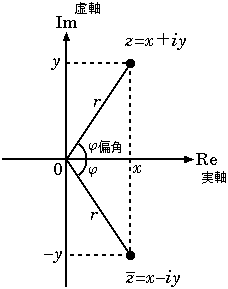
\includegraphics[width=4cm]{complex_plane.png}
  \caption{複素数平面(Wikipediaから引用)}
\end{figure}
\end{block}
\end{frame}

\section{複素指数函数と複素三角函数}

\section{Mandelbrot集合}



\end{document}
